%
% section 3.4
%
\section{Διευθύνσεις IP και Ονοματολογία}
\label{sec:sec34}

Όπως γνωρίζουμε, οι διευθύνσεις στο IPv4 είναι στην πραγματικότητα δυαδικοί αριθμοί των 32bit.  Ωστόσο σχεδόν πάντα τους χωρίζουμε σε οκτάδες ψηφίων και τους γράφουμε με δεκαδικούς αριθμούς χωρισμένους μεταξύ τους με τελείες, ώστε να τους θυμόμαστε πιο εύκολα. Αυτός ο τρόπος γραφής ονομάζεται \emph{dotted decimal}.

Συγκρίνετε για παράδειγμα τη διεύθυνση:

\begin{center}
\begin{verbatim}
192.168.1.2
\end{verbatim}
\end{center}

με την αντίστοιχη δυαδική:

\begin{center}
\begin{verbatim}
‭11000000‬.‭10101000‬.00000001.00000010
\end{verbatim}
\end{center}

Όμως ακόμα και με την δεκαδική αναπαράσταση, είναι απίθανο για ένα άνθρωπο να απομνημονεύσει πάνω από μερικές διευθύνσεις. Αν και οι υπολογιστές δεν έχουν κανένα πρόβλημα στην αποθήκευση αριθμών, οι άνθρωποι τα πηγαίνουν καλύτερα με τα ονόματα: σπάνια θυμόμαστε για παράδειγμα τους αριθμούς τηλεφώνων όλων των φίλων μας. Τυπικά χρησιμοποιούμε το όνομα τους και αναζητούμε το τηλέφωνο τους σε ένα κατάλογο (σημειωματάριο, τις επαφές στο κινητό μας κλπ). 

Αν και το πρωτόκολλο IP χρησιμοποιεί μόνο τις διευθύνσεις, για τη δική μας ευκολία χρειάζεται κάποιο σύστημα αντίστοιχο με τον τηλεφωνικό κατάλογο: να μπορούμε να αναφερθούμε σε ένα υπολογιστή με το όνομα του και με κάποιο τρόπο να αντιστοιχιστεί στην πραγματική διεύθυνση IP.

Στην αρχή της ανάπτυξης του Internet, το πλήθος των υπολογιστών ήταν πολύ μικρό και συνήθως οι ίδιοι οι ``χρήστες'' του Διαδικτύου ήταν και οι διαχειριστές των μηχανημάτων. Στα περισσότερα μηχανήματα δίνονταν απλώς ένα \emph{μονολεκτικό όνομα}. Θα έπρεπε όμως με κάποιο τρόπο να υπάρχει μια λίστα που να αντιστοιχεί αυτά τα ονόματα σε διευθύνσεις. Με τη λίστα αυτή οι άνθρωποι θα μπορούσαν να χρησιμοποιούν τα ονόματα, ενώ τα πρωτόκολλα θα τη συμβουλεύονταν για να βρουν την αριθμητική διεύθυνση. Το ρόλο αυτής της λίστας ανέλαβε το αρχείο \emph{hosts}.

\begin{inthebox}
\textbf{Σημείωση:} Το βιβλίο σας το αναφέρει ως HOSTS.TXT -- ίσως για να τονίσει ότι πρόκειται για αρχείο κειμένου. Στην πραγματικότητα, δεν έχει την κατάληξη .TXT σε κανένα λειτουργικό σύστημα (ούτε στα Windows). Είναι όμως κοινό αρχείο κειμένου που μπορούμε να το ανοίξουμε με το Σημειωματάριο. Για να αλλάξουμε κάποια καταχώριση σε αυτό χρειάζονται δικαιώματα διαχειριστή.\\
\end{inthebox}

Κάθε φορά που προστίθεται ένα υπολογιστής στο δίκτυο, πρέπει να προστεθεί η αντίστοιχη εγγραφή στο αρχείο αυτό, με μορφή:

<διεύθυνση IP>	 \hfill	 <όνομα υπολογιστή>

το πρόβλημα όμως είναι ότι αυτό το αρχείο θα πρέπει να υπάρχει -- ενημερωμένο -- σε κάθε υπολογιστή του δικτύου. Αρχικά, όταν το Internet αποτελούνταν από λίγα μηχανήματα, οι διαχειριστές αντάλλαζαν μεταξύ τους το αρχείο κάθε φορά που γίνονταν κάποια αλλαγή και εγκαθιστούσαν τη νέα έκδοση στα μηχανήματα που διαχειρίζονταν. Προφανώς μια τέτοια τακτική δεν μπορεί να λειτουργήσει όταν διαχειριζόμαστε ένα δίκτυο με περισσότερα από λίγες δεκάδες μηχανήματα.

Το αρχείο αυτό πάντως εξακολουθεί να υπάρχει μέχρι σήμερα, αν και η χρήση του είναι περιορισμένη.

\begin{figure}[!ht]
 \centering
 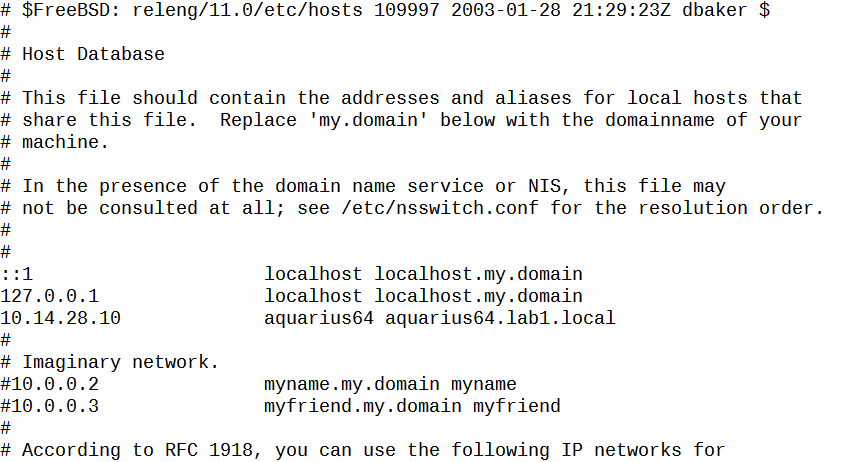
\includegraphics[width=0.85\textwidth]{images/chapter3/3-20}
 \caption {\textsl{Απόσπασμα Αρχείου hosts σε Λειτουργικό UNIX (FreeBSD)}}
 \label{3-20}
\end{figure}

\begin{inthebox}
\textbf{Σημείωση:} Ακόμα και σήμερα τα περισσότερα συστήματα είναι ρυθμισμένα πρώτα να συμβουλεύονται το αρχείο hosts και μετά τις υπόλοιπες υπηρεσίες ονομάτων (τυπικά το DNS). Έτσι μπορούμε να χρησιμοποιήσουμε αυτό το αρχείο για να αποκλείσουμε διευθύνσεις (blacklisting) στις οποίες δεν θέλουμε να συνδεθεί ο υπολογιστής μας. Αρκεί να προσθέσουμε μια γραμμή που να παραπέμπει το αντίστοιχο όνομα σε μια ψεύτικη διεύθυνση ή (συνήθως) στο localhost -- 127.0.0.1\\
\end{inthebox}

Στα Windows θα βρείτε το αρχείο αυτό στην τοποθεσία:

\begin{verbatim}
%SystemRoot%\System32\drivers\etc\hosts
\end{verbatim}

(τυπικά το SystemRoot είναι συνήθως ο φάκελος C:\textbackslash{}Windows). Σε μηχανήματα UNIX/Linux το αρχείο βρίσκεται στη θέση /etc/hosts. Μπορείτε να δείτε ένα υπόδειγμα αρχείου hosts στο σχήμα \ref{3-20}.

Καθώς ο αριθμός των διασυνδεδεμένων στο Internet υπολογιστών αυξάνονταν με ραγδαίο ρυθμό, έγινε γρήγορα φανερό ότι ούτε το αρχείο hosts ούτε ο επίπεδος χώρος ονομάτων (απλό όνομα υπολογιστή, χωρίς τομέα) θα μπορούσαν να αντεπεξέλθουν. Σχετικά νωρίς (1983) προτάθηκε και υλοποιήθηκε η \emph{Υπηρεσία Ονομάτων Περιοχών ή DNS, Domain Name System}. Στο DNS, το σύστημα ονομάτων δεν είναι επίπεδο αλλά \emph{ιεραρχικά δομημένο και οργανωμένο σε περιοχές και υποπεριοχές σε διάφορα επίπεδα}. Στο κατώτερο επίπεδο, στο αριστερό μέρος βρίσκεται το όνομα του υπολογιστή. Η διαδικασία μετάφρασης -- αντιστοίχισης των ονομάτων σε διευθύνσεις ονομάζεται \emph{ανάλυση ονομάτων} (name resolve) και το κομμάτι του λογισμικού που εκτελεί αυτή τη διαδικασία \emph{name resolver}.

Η μορφή ενός ονόματος στο DNS είναι:

\begin{centering}
υπολογιστής.υποπεριοχή\_n. \ldots{} .υποπεριοχή\_1.περιοχή\_TLD
\end{centering}

όπου TLD = Top Level Domain (περιοχή ανώτατου επιπέδου).

για παράδειγμα στη διεύθυνση:

\begin{centering}
joshua.freebsdgr.org
\end{centering}

Το \textbf{joshua} είναι το όνομα του υπολογιστή, το \textbf{.freebsdgr} είναι η υποπεριοχή και το \textbf{.org} είναι η περιοχή ανώτατου επιπέδου.

Το σύστημα DNS δουλεύει ως μια μεγάλη κατανεμημένη και ιεραρχικά δομημένη βάση δεδομένων. Τμήματα της βάσης βρίσκονται σε διάφορους εξυπηρετητές της υπηρεσίας, οι οποίοι είναι υπεύθυνοι να απαντούν σε ερωτήματα για συγκεκριμένες περιοχές και υποπεριοχές. Θα εξετάσουμε αναλυτικότερα το DNS στην ενότητα \ref{sec:sec61}. 

Μπορείτε να βρείτε περισσότερες πληροφορίες στα \href{https://www.ietf.org/rfc/rfc882.txt}{RFC882}, \href{https://www.ietf.org/rfc/rfc883.txt}{RFC883}, \href{https://www.ietf.org/rfc/rfc1034.txt}{RFC1034} και \href{https://www.ietf.org/rfc/rfc1035.txt}{RFC1035}.